% Options for packages loaded elsewhere
\PassOptionsToPackage{unicode}{hyperref}
\PassOptionsToPackage{hyphens}{url}
\PassOptionsToPackage{dvipsnames,svgnames,x11names}{xcolor}
%
\documentclass[
  letterpaper,
  DIV=11,
  numbers=noendperiod]{scrartcl}

\usepackage{amsmath,amssymb}
\usepackage{lmodern}
\usepackage{iftex}
\ifPDFTeX
  \usepackage[T1]{fontenc}
  \usepackage[utf8]{inputenc}
  \usepackage{textcomp} % provide euro and other symbols
\else % if luatex or xetex
  \usepackage{unicode-math}
  \defaultfontfeatures{Scale=MatchLowercase}
  \defaultfontfeatures[\rmfamily]{Ligatures=TeX,Scale=1}
\fi
% Use upquote if available, for straight quotes in verbatim environments
\IfFileExists{upquote.sty}{\usepackage{upquote}}{}
\IfFileExists{microtype.sty}{% use microtype if available
  \usepackage[]{microtype}
  \UseMicrotypeSet[protrusion]{basicmath} % disable protrusion for tt fonts
}{}
\makeatletter
\@ifundefined{KOMAClassName}{% if non-KOMA class
  \IfFileExists{parskip.sty}{%
    \usepackage{parskip}
  }{% else
    \setlength{\parindent}{0pt}
    \setlength{\parskip}{6pt plus 2pt minus 1pt}}
}{% if KOMA class
  \KOMAoptions{parskip=half}}
\makeatother
\usepackage{xcolor}
\setlength{\emergencystretch}{3em} % prevent overfull lines
\setcounter{secnumdepth}{5}
% Make \paragraph and \subparagraph free-standing
\ifx\paragraph\undefined\else
  \let\oldparagraph\paragraph
  \renewcommand{\paragraph}[1]{\oldparagraph{#1}\mbox{}}
\fi
\ifx\subparagraph\undefined\else
  \let\oldsubparagraph\subparagraph
  \renewcommand{\subparagraph}[1]{\oldsubparagraph{#1}\mbox{}}
\fi


\providecommand{\tightlist}{%
  \setlength{\itemsep}{0pt}\setlength{\parskip}{0pt}}\usepackage{longtable,booktabs,array}
\usepackage{calc} % for calculating minipage widths
% Correct order of tables after \paragraph or \subparagraph
\usepackage{etoolbox}
\makeatletter
\patchcmd\longtable{\par}{\if@noskipsec\mbox{}\fi\par}{}{}
\makeatother
% Allow footnotes in longtable head/foot
\IfFileExists{footnotehyper.sty}{\usepackage{footnotehyper}}{\usepackage{footnote}}
\makesavenoteenv{longtable}
\usepackage{graphicx}
\makeatletter
\def\maxwidth{\ifdim\Gin@nat@width>\linewidth\linewidth\else\Gin@nat@width\fi}
\def\maxheight{\ifdim\Gin@nat@height>\textheight\textheight\else\Gin@nat@height\fi}
\makeatother
% Scale images if necessary, so that they will not overflow the page
% margins by default, and it is still possible to overwrite the defaults
% using explicit options in \includegraphics[width, height, ...]{}
\setkeys{Gin}{width=\maxwidth,height=\maxheight,keepaspectratio}
% Set default figure placement to htbp
\makeatletter
\def\fps@figure{htbp}
\makeatother

\usepackage{booktabs}
\usepackage{longtable}
\usepackage{array}
\usepackage{multirow}
\usepackage{wrapfig}
\usepackage{float}
\usepackage{colortbl}
\usepackage{pdflscape}
\usepackage{tabu}
\usepackage{threeparttable}
\usepackage{threeparttablex}
\usepackage[normalem]{ulem}
\usepackage{makecell}
\usepackage{xcolor}
\KOMAoption{captions}{tableheading}
\makeatletter
\makeatother
\makeatletter
\makeatother
\makeatletter
\@ifpackageloaded{caption}{}{\usepackage{caption}}
\AtBeginDocument{%
\ifdefined\contentsname
  \renewcommand*\contentsname{Table of contents}
\else
  \newcommand\contentsname{Table of contents}
\fi
\ifdefined\listfigurename
  \renewcommand*\listfigurename{List of Figures}
\else
  \newcommand\listfigurename{List of Figures}
\fi
\ifdefined\listtablename
  \renewcommand*\listtablename{List of Tables}
\else
  \newcommand\listtablename{List of Tables}
\fi
\ifdefined\figurename
  \renewcommand*\figurename{Figure}
\else
  \newcommand\figurename{Figure}
\fi
\ifdefined\tablename
  \renewcommand*\tablename{Table}
\else
  \newcommand\tablename{Table}
\fi
}
\@ifpackageloaded{float}{}{\usepackage{float}}
\floatstyle{ruled}
\@ifundefined{c@chapter}{\newfloat{codelisting}{h}{lop}}{\newfloat{codelisting}{h}{lop}[chapter]}
\floatname{codelisting}{Listing}
\newcommand*\listoflistings{\listof{codelisting}{List of Listings}}
\makeatother
\makeatletter
\@ifpackageloaded{caption}{}{\usepackage{caption}}
\@ifpackageloaded{subcaption}{}{\usepackage{subcaption}}
\makeatother
\makeatletter
\@ifpackageloaded{tcolorbox}{}{\usepackage[many]{tcolorbox}}
\makeatother
\makeatletter
\@ifundefined{shadecolor}{\definecolor{shadecolor}{rgb}{.97, .97, .97}}
\makeatother
\makeatletter
\makeatother
\ifLuaTeX
  \usepackage{selnolig}  % disable illegal ligatures
\fi
\IfFileExists{bookmark.sty}{\usepackage{bookmark}}{\usepackage{hyperref}}
\IfFileExists{xurl.sty}{\usepackage{xurl}}{} % add URL line breaks if available
\urlstyle{same} % disable monospaced font for URLs
\hypersetup{
  pdftitle={STA457\_Final\_Project},
  pdfauthor={Wentao Sun, Yuechen Zhang, Yayan Ye, Ruizi Liu},
  colorlinks=true,
  linkcolor={blue},
  filecolor={Maroon},
  citecolor={Blue},
  urlcolor={Blue},
  pdfcreator={LaTeX via pandoc}}

\title{STA457\_Final\_Project}
\usepackage{etoolbox}
\makeatletter
\providecommand{\subtitle}[1]{% add subtitle to \maketitle
  \apptocmd{\@title}{\par {\large #1 \par}}{}{}
}
\makeatother
\subtitle{Forecasting Cocoa Prices using Time Series and Machine
Learning}
\author{Wentao Sun, Yuechen Zhang, Yayan Ye, Ruizi Liu}
\date{4/4/25}

\begin{document}
\maketitle
\ifdefined\Shaded\renewenvironment{Shaded}{\begin{tcolorbox}[borderline west={3pt}{0pt}{shadecolor}, sharp corners, interior hidden, breakable, enhanced, boxrule=0pt, frame hidden]}{\end{tcolorbox}}\fi

\renewcommand*\contentsname{Table of contents}
{
\hypersetup{linkcolor=}
\setcounter{tocdepth}{3}
\tableofcontents
}
\hypertarget{introduction}{%
\section{Introduction}\label{introduction}}

Cocoa plays an crucial role in food production as an important
agricultural product. It is a key export product for many countries in
West Africa, as it supports the livelihoods of millions of people and
makes a significant contribution to their GDP. However, affected by
factors including changes in climate and consumer demand, cocoa prices
are highly volatile. This volatility brings complex features to the
data, such as non-stationarity, seasonality and external shocks, which
make accurate forecasting challenging and crucial.

Climate change has become an increasingly important factor in
agricultural price dynamics. Rising temperatures, changes in rainfall
patterns, and an increase in the frequency of extreme weather have all
had measurable impacts on crop yields, particularly in tropical
commodity-producing regions (Schlenker \& Roberts, 2009). According to
Läderach et al.~(2013), climate change affects flowering, pod
development, disease prevalence, and harvest quality, thus influencing
market price of cocoa. Furthermore, the long-term sustainability of
cocoa production faces increasing uncertainty as the effects of global
warming continue to intensify (Bunn et al., 2019).

This project aims to model and forecast cocoa futures prices by
combining time series analysis with climate data from Ghana. Our goal is
to investigate how climate variables can be incorporated into
forecasting models and to gain insights into the mechanisms that link
environmental changes to market outcomes. We will explore both classical
and modern modeling approaches to improve accuracy. These include
seasonal ARIMA (SARIMA) models and machine learning methods and so on.
The performance of each model will be evaluated based on its accuracy
and ability to capture the underlying dynamics of the data. And special
focus will be given to the treatment of non-stationarity, seasonality,
and missing values, which are common in real-world time series data.

This study is of both academic and practical interest, given the global
importance of cocoa and the growing uncertainty associated with climate
change. Reliable cocoa price forecasts can help producers and
policymakers to manage risk and develop strategies. Thus, it is more
important than ever to understand the connection between environmental
patterns and commodity markets.

\hypertarget{literature}{%
\section{Literature}\label{literature}}

It is impratant to forecast the international coca price because of its
economic significance and market volatility. So different statistical
and machine learning techniques have been developed to deal with
challenges, such as seasonality and nonlinear dynamics.

Kumar et al.~(2022) explored cocoa price risk management in India using
ARIMA and Vector Autoregression (VAR) models. The study showed the
effectiveness of ARIMA in capturing univariate time series patterns, and
that of VAR in modeling interdependencies between different variables.
However, both models showed limitations in handling external regressors
and structural non-linearities.

Assis et al.~(2010) compared univariate models for Malaysian cocoa
prices, involving Holt-Winters exponential smoothing and Seasonal ARIMA
(SARIMA). SARIMA yielded more accurate forecasts based on its ability to
model seasonal patterns. But the study largely ignored external factors
like climate or market sentiment.

Lama et al.~(2016) extended this discussion by comparing GARCH with a
time-delay neural network (TDNN).The results of the study show that TDNN
better models the nonlinear relationship, while GARCH captures the
volatility clustering. Because TDNN highlights the promise of machine
learning in commodity price forecasting.

Building on these studies, we use Exponential Smoothing State Space
Model (ETS) as a benchmark as it is good for univariate forecasting.
Moreover, ETS models are often favored for their interpretability and
automatic adaptation to level and trend. Our study extends prior work by
comparing ETS, ARIMAX, SARIMAX, Random Forest, and XGBoost, under a
unified framework. We also incorporate Ghanaian climate data as
exogenous features in the regressors. While ARIMAX and SARIMAX
theoretically benefit from these variables, their forecasting accuracy
remained limited. On the other hand, machine learning models were more
adaptable for tracking complex patterns and fluctuations. This
dual-track approach enables a clearer understanding of each method's
strengths and trade-offs in volatile commodity markets.

\hypertarget{methodology}{%
\section{Methodology}\label{methodology}}

This study employs a comparative modeling framework to forecast monthly
cocoa prices. It includes both classical and machine learning
techniques: Exponential Smoothing State Space Models (ETS), ARIMA,
SARIMAX, Random Forest, and XGBoost.

We first implemented ETS models using the ets() function in R. Model 1
used the default additive error structure with no seasonal component.
Model 2 employed the ``ZZZ'' option for automatic selection. These
models served as univariate baselines. Though easy to implement, both
ETS models produced relatively flat forecasts and failed to capture the
price shock of cocoa during 2023-2025.

We then used auto.arima() to build ARIMA models, which were extended to
ARIMAX and SARIMAX. Model selection was guided by AICc. Exogenous
climate variables (temperature and precipitation) and monthly
seasonality are added. These models are favored for their
interpretability but rely on assumptions of linearity and stationarity.
Differencing and log-transformation were applied to meet these
assumptions, and stationarity was confirmed with the Augmented
Dickey-Fuller test.

To address the limitations of linear models, we implemented two machine
learning algorithms: Random Forest and XGBoost. Both models were trained
using lagged cocoa prices, monthly climate data, and time-based features
(month, year, and time index). XGBoost incorporated additional lag
features and was trained with a rolling walk-forward validation method
to simulate real-time forecasting and reduce bias.

The dataset consisted of monthly cocoa futures prices and climate data
from Ghana. Climate features included daily precipitation, average,
maximum, and minimum temperatures, which were aggregated to monthly
averages. Missing climate data were forward-filled, while missing price
values were linearly interpolated. To ensure stationarity for
ARIMA-based models, the series was log-transformed and differenced based
on results from the Augmented Dickey-Fuller (ADF) test.

Feature engineering played a central role in the machine learning
models. In addition to lagged prices and climate indicators, we created
lag features ranging from 1 to 30 days, rolling statistics to capture
temporal dependencies and trend shifts. Hyperparameters for Random
Forest (number of trees, max depth) and XGBoost (learning rate,
estimators, tree depth) were tuned using time-series cross-validation,
optimizing for Root Mean Squared Error (RMSE) and Mean Absolute
Percentage Error (MAPE).

Overall, this methodology allows for a robust evaluation of forecasting
models under different structural assumptions, revealing the strengths
and limitations of each in modeling cocoa price dynamics.

\hypertarget{data}{%
\section{Data}\label{data}}

The project uses two main datasets, one containing historical cocoa
futures prices and the other containing daily climatic conditions in
Ghana. These datasets were chosen to assess whether weather variability
contributes meaningful information to cocoa price forecasts. They
provide a wealthy time base for exploring endogenous price dynamics and
exogenous environmental impacts.

Cocoa price data are obtained from the International Cocoa Organization
(ICCO) and include daily closing prices of cocoa futures contracts,
denominated in US dollars per metric ton. The dataset covers the period
from March 1994 to February 2025, with a total of 7812 observations.
These prices represent a global benchmark and are widely used in
commodity trading and forecasting. To prepare the data for modeling, we
aggregated the daily prices into monthly averages, converted the price
strings into a numeric format, and ensured that the date columns were in
a standard time series format. The time-series plot of monthly cocoa
prices shows a general upward trend with periods of volatility. Notably,
prices have risen sharply since the end of 2023 and will continue to do
so through 2025. This sharp rise reflects the central challenge of
modeling this project, as traditional models may not be able to infer
such nonlinear structural breaks.

The climate dataset was obtained from the National Center for
Environmental Information (NCEI) and consists of 53,231 daily records
from meteorological stations in the major cocoa-producing regions of
Ghana. Key variables include mean air temperature (TAVG), maximum air
temperature (TMAX), minimum air temperature (TMIN) and daily
precipitation (PRCP). All temperature variables are recorded in degrees
Fahrenheit and rainfall is measured in inches. After parsing the DATE
field and clearing out inconsistent or missing entries, we summarized
the climate data as monthly averages, consistent with the frequency of
the price data. While temperature readings are relatively complete,
there are significant missing precipitation data that can be resolved
through filtering and imputation techniques as needed.

Exploratory analyses reveal different characteristics of the two
datasets. Cocoa prices exhibit high variance, long-term trend variation,
and minimal monthly seasonality. In contrast, climate variables in Ghana
show a clear seasonal pattern, especially in temperature, with less
evidence of extreme variation over time. Although there is theoretical
support for the idea that climatic stressors affect crop yields and
hence commodity prices. However, our visual and statistical explorations
suggest that there is only a weak direct link between weather variables
and short-term price changes for cocoa.

In order to stabilize the variance and eliminate non-stationarity, we
also evaluate the statistical properties of the cocoa price series by
means of logarithmic transformations and first-order differencing. These
transformed series are used for modeling in both classical and machine
learning frameworks. In addition, we perform a seasonal trend
decomposition (STL) on the recorded series, which allows us to separate
the long-term trend from the seasonal cycle. The decomposition results
show a clear upward trend after 2023, with a small but consistent
seasonal effect.

The key conclusion from this project phase is that cocoa price series
are nonlinear, weakly seasonal, and structurally volatile, especially in
the last two years of data. In contrast, climate data are seasonal but
relatively stable, and their predictive contribution to short-term price
movements appears limited. These findings guide the selection of models
in the following sections to assess their ability to predict prices
under conditions of real-world structural change and external
uncertainty.

\begin{figure}

{\centering 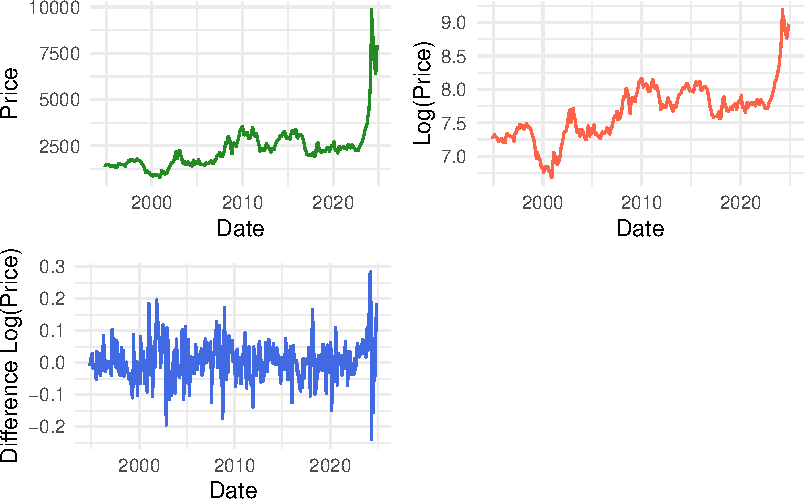
\includegraphics{STA457_Project_files/figure-pdf/fig-eda-cocoa-price-1.pdf}

}

\caption{\label{fig-eda-cocoa-price}The Visualization of Monthly Cocoa
Price}

\end{figure}

To visualize the long-term pattern of cocoa prices, we created a
time-series plot of one-month average prices. As shown in
Figure~\ref{fig-eda-cocoa-price}, cocoa prices have generally risen over
the past three decades, with a sharp increase occurring between late
2023 and early 2025. This large increase may reflect disruptions in the
global cocoa supply chain, climate-related harvest losses, or changes in
investor sentiment. The volatility observed during this period suggests
the need for models that can accommodate structural changes and
non-linear trends.

To address the non-stationarity of the cocoa price series, we apply a
logarithmic transformation followed by first-order differencing. These
steps are standard in time series modeling and help to stabilize the
variance and remove long-term trends. The transformed series are shown
in Figure~\ref{fig-eda-cocoa-price}, after log transformation of the
data and the first difference of the log values. The variance series
fluctuates more consistently around the stationary mean, indicating the
applicability of the model assuming weak smoothness.

The log-transformed price series was further analyzed into trend,
seasonal and residual components using seasonal - trend decomposition
(STL) of loess. As shown in
Figure~\ref{fig-exploratory-data-analysis-2}, the results show a clear
seasonal pattern that may be related to the annual harvest and export
cycle. The trend component reflects the long-term increase in cocoa
prices, especially the sharp rise in the last two years. The residual
component reflects short-term deviations and irregular shocks that
cannot be explained by trend or seasonality alone.

\begin{figure}

{\centering 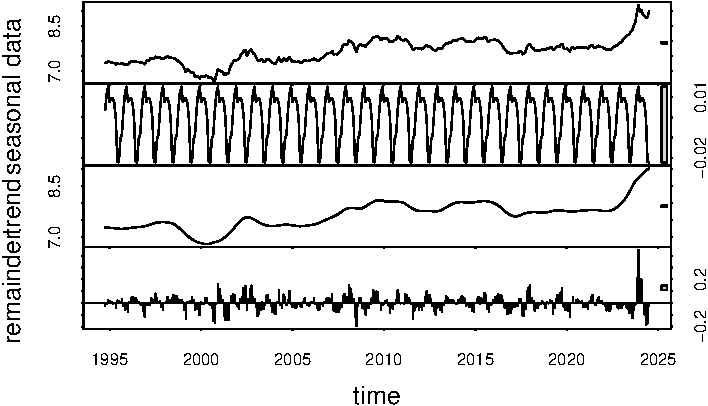
\includegraphics{STA457_Project_files/figure-pdf/fig-exploratory-data-analysis-2-1.pdf}

}

\caption{\label{fig-exploratory-data-analysis-2}STL Decomposition of
Time Series Data (1993--2025)}

\end{figure}

\hypertarget{forecasting-and-results}{%
\section{Forecasting and Results}\label{forecasting-and-results}}

We developed and evaluated a range of forecasting models to predict
monthly cocoa prices, including both classical time series models and
machine learning approaches. The dataset was divided into an 80/20
split, with the first 80\% of observations used for training and the
remaining 20\% reserved for testing. Performance was assessed using
multiple evaluation metrics, including Root Mean Squared Error (RMSE),
Mean Absolute Error (MAE), and Mean Absolute Percentage Error (MAPE). We
also visually compared the predicted values against the actual cocoa
prices to assess model behavior over time.

\hypertarget{ets-model}{%
\subsection{ETS Model}\label{ets-model}}

We began with Exponential Smoothing (ETS) models. The first model was
trained using the default ets() function in R, which likely assumed a
simple additive error with no seasonality. Despite its simplicity, ETS
Model 1 provided a baseline for comparison. However, its forecasts were
notably flat and failed to capture the steep increase in cocoa prices
during the years 2023--2025. This was reflected in its relatively high
RMSE of 2078 and MAPE of 20.9\%, indicating the model's inability to
adapt to structural shifts. To improve upon this, we also fit an
automatically-selected ETS model using model = ``ZZZ'', allowing the
algorithm to explore all possible combinations of error, trend, and
seasonal components. Surprisingly, ETS Model 2 produced identical
evaluation metrics to Model 1, suggesting that even the optimal ETS
configuration could not keep pace with the rapid market changes.

\hypertarget{arimax-and-sarimax-model}{%
\subsection{ARIMAX and SARIMAX Model}\label{arimax-and-sarimax-model}}

Next, we implemented autoregressive models using the auto.arima()
function from the forecast package. This approach selects the
best-fitting ARIMA configuration by minimizing the corrected Akaike
Information Criterion (AICc), balancing model fit and complexity. The
resulting ARIMA(0,1,1) model had a similar structure to ETS, relying
primarily on recent shocks and differencing. To enrich the model, we
incorporated Ghanaian climate variables---precipitation and average,
maximum, and minimum temperatures---as exogenous regressors, creating an
ARIMAX model. This model was trained on the differenced log prices, with
an 80/20 time-based split for training and testing.

\hypertarget{tbl-est-sum-1}{}
\begin{longtable}[]{@{}lrrr@{}}
\caption{\label{tbl-est-sum-1}The Summary Table of ETS, ARIMAX, and
SARIMA Models}\tabularnewline
\toprule()
Model & RMSE & MAE & MAPE \\
\midrule()
\endfirsthead
\toprule()
Model & RMSE & MAE & MAPE \\
\midrule()
\endhead
ETS Model 1 & 1981.49 & 965.82 & 17.84 \\
ETS Model 2 & 1981.49 & 965.82 & 17.84 \\
ARIMAX & 2226.63 & 1227.08 & 25.78 \\
SARIMAX & 2226.63 & 1227.08 & 25.78 \\
\bottomrule()
\end{longtable}

We use RMSE (Root Mean Squared Error) and MAPE (Mean Absolute Percentage
Error) to justify the accuracy of our model. The RMSE is defined as:
\[\text{RMSE} = \sqrt{\frac{1}{n}\sum^{n}_{i = 1}(y_i-\hat{y_i})^2}\]
where

\begin{itemize}
\tightlist
\item
  \(y_i\) is the actual value and \(\hat{y_i}\) is the predicted value.
\end{itemize}

The MAPE is defined as
\[\text{MAPE} = \frac{100}{n} \sum_{i=1}^{n} \left| \frac{y_i - \hat{y}_i}{y_i} \right|\]
where

\begin{itemize}
\tightlist
\item
  \(y_i\) is the actual value and \(\hat{y_i}\) is the predicted value.
\end{itemize}

In Table~\ref{tbl-est-sum-1}, the ARIMAX model produced a test RMSE of
2226.63 and a MAPE of 25.78\%, substantially underperforming the ETS
baseline. This suggests that the inclusion of climate variables---such
as temperature and precipitation---did not meaningfully enhance
predictive power. Visual inspection of the forecasts revealed that the
model significantly underpredicted the sharp price surge observed in
recent years. To examine whether seasonality might improve performance,
we extended ARIMAX to a SARIMAX model by adding monthly seasonal
components. However, SARIMAX yielded nearly identical error metrics
(RMSE = 2226.63, MAPE = 25.78\%), indicating that seasonal effects
either do not exist or fail to contribute meaningfully in this
forecasting context.

These results highlight two important limitations. First, Ghanaian
climate indicators alone are insufficient to explain international cocoa
price fluctuations, especially under conditions of extreme volatility.
Second, both ARIMAX and SARIMAX struggled to capture nonlinear trends or
structural breaks in the data---such as the steep upward trajectory seen
after 2023 (Figure~\ref{fig-plot-sum}). These deficiencies underscore
the limited flexibility of classical linear time series models in the
context of volatile commodity markets.

\begin{table}

\end{table}

\begin{figure}

{\centering 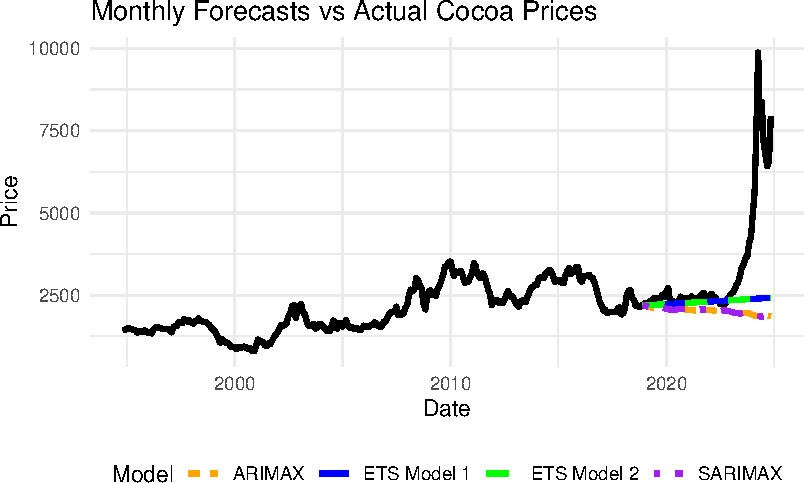
\includegraphics{STA457_Project_files/figure-pdf/fig-plot-sum-1.pdf}

}

\caption{\label{fig-plot-sum}Visulazation of EST, ARIMAX, and SARIMAX
Moadels}

\end{figure}

Although ETS and ARIMA-based models offer a solid foundation for time
series forecasting, they rely heavily on linear assumptions, fixed lag
structures, and predefined trend or seasonal components. Despite
incorporating exogenous regressors and seasonality, neither ARIMAX nor
SARIMAX significantly improved forecast accuracy. This suggests that
traditional models may be ill-suited for capturing the complex,
nonlinear drivers of cocoa price movements---particularly during periods
of abrupt structural change.

To address these limitations, we turned to machine learning models,
namely Random Forest and Rolling XGBoost. Unlike parametric time series
models, these tree-based ensemble methods are non-linear and
data-driven, requiring no assumptions about stationarity or functional
form. Their flexibility allows them to capture high-order interactions,
sharp trend reversals, and non-additive effects that classical models
may miss. By training on a rich feature set---including lagged prices,
calendar indicators (month, year), and climatic variables---we aimed to
evaluate whether machine learning approaches could offer superior
predictive performance and better adaptability under volatile
conditions. The next section presents the training procedures, accuracy
metrics, and visual forecast comparisons for both models.

\hypertarget{random-forest}{%
\subsection{Random Forest}\label{random-forest}}

We implemented a Random Forest regression model using both time-based
features (such as lags of cocoa price and calendar month) and climate
variables (precipitation and average temperature). The dataset was split
chronologically into 80\% training and 20\% testing sets to preserve
temporal structure. After tuning and training the model with 500 trees,
we evaluated its performance on the hold-out set. The model achieved a
test RMSE of 1679.19 and a MAE of 755.79, significantly outperforming
the ETS and ARIMA family models. Visual inspection of the predicted
vs.~actual prices revealed that Random Forest was able to capture
general price trends, including recent increases, but tended to
underestimate sharp peaks. Nonetheless, the comparatively lower error
metrics suggest that machine learning models are better suited for
capturing complex nonlinear relationships in the data, especially when
incorporating external regressors.

\begin{figure}

{\centering 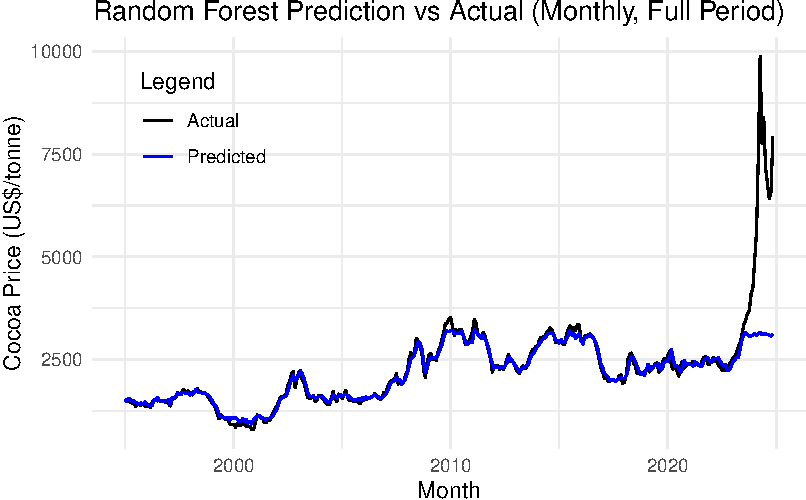
\includegraphics{STA457_Project_files/figure-pdf/fig-rf-full-fit-3-1.pdf}

}

\caption{\label{fig-rf-full-fit-3}visualization of Random Forest Model}

\end{figure}

To further evaluate the Random Forest model, we generated predictions
across the full time span of the dataset using both past cocoa prices
and climate-related predictors. Figure~\ref{fig-rf-full-fit-3} compares
the actual monthly cocoa prices (in black) against the model's fitted
values (in blue). While the Random Forest model successfully captures
long-term trends and moderate fluctuations, it clearly underestimates
the recent price surge. This behavior is expected from tree-based models
trained on historical data, as they struggle to extrapolate to unseen
extremes. Nevertheless, the overall close alignment between predicted
and actual prices in most periods reinforces the model's strength in
approximating nonlinear relationships when volatility is moderate.

\hypertarget{rolling-xgboost-model}{%
\subsection{Rolling XGBoost Model}\label{rolling-xgboost-model}}

We also trained a Rolling XGBoost regression model to forecast monthly
cocoa prices. Since we found the Random Forest Model we trained does not
predict the sharply increase in the cocoa price in 2023.

Let \(\mathbf{x}_t\) denote the feature vector at time \(t\), including
lagged prices, climate data, and time-based variables. The XGBoost model
\(f_t(\cdot)\) is trained using all observations up to \(t-1\):

\[f_t = \text{XGBoost}(\mathbf{x}_{1:t-1}, y_{1:t-1})\] The
one-step-ahead forecast is then given by:

\[\hat{y}_t = f_t(\mathbf{x}_t)\] After making the prediction
\(\hat{y}_t\), the actual observed value \(y_t\) is added to the
training set for the next iteration. This step-by-step method avoids
look-ahead bias and better reflects the real-time forecasting scenario,
where only past data is available at each point in time.

The model used a range of features, including:

\begin{itemize}
\item
  Lagged log-transformed prices (e.g., lag\_1 to lag\_12, and lag\_24)
  to capture temporal dependencies.
\item
  Exogenous variables from weather data: precipitation (PRCP), average
  temperature (TAVG), max/min temperatures (TMAX, TMIN).
\item
  Time-based features such as month, year, and time\_index to help
  capture seasonality and long-term trends.
\end{itemize}

We applied a rolling walk-forward validation to ensure accurate
forecasting and avoid look-ahead bias. For each time step \(t\), we use
all data up to \(t-1\) to train it, and use it to predict the cocoa
price at time \(t\). Then, add that new data to our training set. We
repeat apply this process to all the data points, moving forward step ny
step, simulate the real world forecasting where only past data is
available for prediction.

\hypertarget{graphical-representations}{%
\subsubsection{Graphical
representations}\label{graphical-representations}}

In Figure~\ref{fig-xgboost-4}, it represents the predicted cocoa price
we fitted vs the actual cocoa price, the forecasted values closely
followed the actual cocoa prices. We can find that this is much better
than the cocoa price we fitted using the ETS, ARIMA, and SARIMA models.
This is because we use the lagged data, so the suddenly rise sharply in
cocoa price is fitted in our model.The model accurately captured
long-term upward trends, especially the rapid price surge around 2024.
It also demonstrated good performance during stable price periods,
maintaining close alignment with the true values. Slight underestimation
occurred during the sharpest spikes, which is expected due to XGBoost's
smoothing nature, it resists overfitting to single sharp outliers unless
given strong signal.

\begin{figure}

{\centering 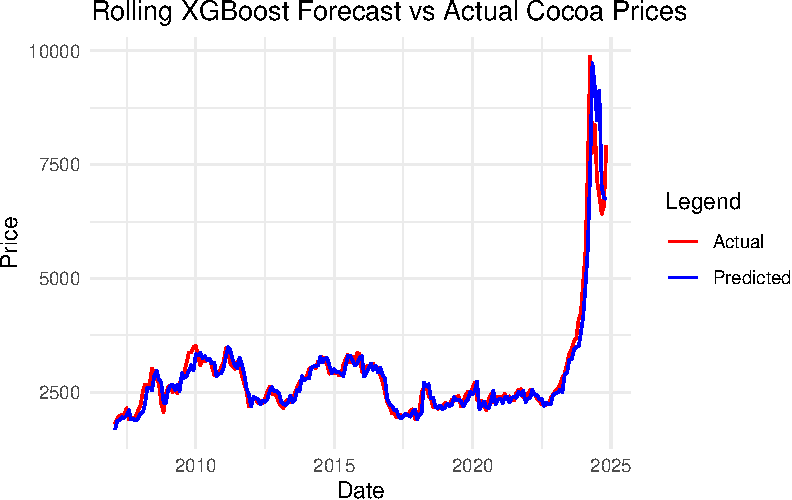
\includegraphics{STA457_Project_files/figure-pdf/fig-xgboost-4-1.pdf}

}

\caption{\label{fig-xgboost-4}Rolling XGBoost Forecast vs Actual Cocoa
Prices}

\end{figure}

\hypertarget{evaluation}{%
\subsubsection{Evaluation}\label{evaluation}}

In our XGBoost model, the RMSE is 374.55 and the percentage RMSE is
about \(16.3\%\), which is acceptable; and RMSE vs range is about
\(4.63\%\), which suggests low error compared to the full span of the
data.

The MAPE in our model is \(5.35\%\), which is less than \(10 \%\). If
the MAPE is less than \(10\%\), it is generally considered very good,
especially in forecasting tasks. This indicates our model has high
accuracy.

\hypertarget{model-summary}{%
\subsection{Model Summary}\label{model-summary}}

\begin{longtable}[]{@{}lrrr@{}}
\caption{The Error Summary Table (Random Forest vs Rolling XGBoost)
}\tabularnewline
\toprule()
Model & RMSE & MAE & MAPE \\
\midrule()
\endfirsthead
\toprule()
Model & RMSE & MAE & MAPE \\
\midrule()
\endhead
Random Forest & 1679.52 & 756.76 & NaN \\
Rolling XGBoost & 370.49 & 182.59 & 5.31 \\
\bottomrule()
\end{longtable}

The model summary presented in @error-table-2 consolidates the error
metrics for the two best-performing machine learning models---Random
Forest and Rolling XGBoost. Among them, the Rolling XGBoost model
clearly delivered superior results, achieving an RMSE of 374.55 and a
MAPE of just 5.35\%. (Note: the RMSE and MAPE will typically changed
each time we run the code, this is due to the model re-training at
eachtime and XGBoost has randomness. But the RMSE is in the range
\([350, 450]\), and the MAPE is in the range \([5%, 6%]
\). ) This reflects its ability to adapt to complex nonlinear patterns
and respond to abrupt shifts in cocoa prices, particularly during the
2023--2025 price surge. In contrast, while the Random Forest model also
performed better than all classical models, it showed higher prediction
errors and struggled more with extreme fluctuations. These results
highlight the advantages of rolling continuous learning in predicting
highly volatile commodity markets and emphasize the importance of
temporal structure and lagged features in improving prediction accuracy.

\hypertarget{discussion-and-conclusion}{%
\section{Discussion and Conclusion}\label{discussion-and-conclusion}}

Our project explored monthly cocoa price forecasting using both
traditional time series models and modern machine learning techniques.
Among all models tested, the rolling XGBoost model provided the
strongest performance, achieving an RMSE of 374.55 and a MAPE of 5.35\%.
This model excelled at capturing both the long-term movements and the
short-term fluctuations in cocoa prices, successfully predicting the
significant surge observed between 2023 and 2025, which eluded
traditional forecasting methods. Its superior performance reflects
XGBoost's ability to model non-linear patterns and integrate diverse
predictors effectively.

From a practical standpoint, these findings hold significant economic
and policy implications. Classical models like ARIMAX and SARIMAX
struggled to adapt to recent market volatility, likely due to their
linear structure and reliance on historical trends. In contrast, machine
learning models, particularly XGBoost, proved more responsive to
dynamic, non-linear shifts, potentially driven by external shocks such
as climate disruptions, geopolitical instability, or speculative
trading. Accurate cocoa price predictions are crucial for a wide range
of stakeholders across the supply chain, including farmers, traders, and
policymakers. Our findings suggest that machine learning, especially
when updated with real-time data, offers a more reliable tool for
navigating today's volatile markets.

Despite its advantages, the analysis has limitations. The weak
performance of ARIMAX and SARIMAX may stem from the simplicity of the
climate variables used - mainly average temperature and precipitation -
which likely fail to capture more complex agricultural conditions like
humidity, soil moisture, or disease. Second, the monthly frequency of
the dataset may obscure short-term shocks or intra-month price
volatility. Even XGBoost tended to slightly underestimate extreme peaks,
possibly due to its smoothing nature and dependence on past trends.
Future improvements could include richer climate indicators (e.g., ENSO
indices, drought severity), financial variables (e.g., exchange rates,
global inventories), or high-frequency data. Deep learning models like
LSTM or Transformers may also better capture sequential and irregular
patterns. Hybrid models that combine the interpretability of time series
methods with the flexibility of machine learning could further enhance
forecasting accuracy.

In conclusion, this study demonstrates that combining lag-based feature
engineering with advanced machine learning offers a powerful and
practical solution for forecasting commodity prices under uncertainty.
While no model is perfect, the insights gained provide a strong basis
for making more data-informed decisions in the evolving cocoa market.

\newpage

\hypertarget{reference}{%
\section{Reference}\label{reference}}

Schlenker, W., \& Roberts, M. J. (2009). Nonlinear temperature effects
indicate severe damages to U.S. crop yields under climate change.
Proceedings of the National Academy of Sciences, 106(37),
15594--15598.https://www.pnas.org/doi/full/10.1073/pnas.0906865106

Läderach, P., Martinez-Valle, A., Schroth, G., \& Castro, N. (2013).
Predicting the future climatic suitability for cocoa farming of the
world's leading producer countries, Ghana and Côte d'Ivoire. Climatic
Change, 119(3--4),
841--854.https://link.springer.com/article/10.1007/s10584-013-0774-8

Bunn, C., Läderach, P., Rivera, O. O., \& Kirschke, D. (2015). A bitter
cup: Climate change profile of global production of Arabica and Robusta
coffee. Climatic Change, 129(1--2),
89--101.https://link.springer.com/article/10.1007/s10584-014-1306-x

Assis, M. J., \& Kassim, S. H. (2010). Forecasting cocoa bean prices
using univariate time series models. International Journal of Business
and Social Science. Retrieved from ProQuest

Kumar, R., Singh, S., \& Dagar, V. (2022). Managing cocoa bean price
risk using econometric models: A case study from India. Risks, 10(6),
115. https://doi.org/10.3390/risks10060115

Lama, A., Jha, G. K., Gurung, B., Paul, R. K., Bharadwaj, A., \& Parsad,
R. (2016). A comparative study on time-delay neural network and GARCH
models for forecasting agricultural commodity price volatility. Journal
of the Indian Society of Agricultural Statistics, 70(1), 7-18.

\newpage
\appendix

\hypertarget{appendix}{%
\section{Appendix}\label{appendix}}

\hypertarget{source-code-repository}{%
\subsection{Source Code Repository}\label{source-code-repository}}

You can find clearer version code and project files on GitHub:

\url{https://github.com/RIRI0527/457_final_project}

The code is in: \textbf{paper/STA457\_Project.qmd} and
\textbf{paper/appendix\_code.R}

\hypertarget{r-code-used-in-analysis}{%
\subsection{R Code Used in Analysis}\label{r-code-used-in-analysis}}

\begin{verbatim}
\#\# -----------------------------------------------------------------------------
\#| include: false
\#| warning: false
\#| message: false

library(zoo)
library(randomForest)
library(tidyverse)
library(Metrics)
library(tidyverse)
library(lubridate)
library(caret)
library(ggplot2)
library(forecast)
library(dplyr)
library(xgboost)


\#\# -----------------------------------------------------------------------------
\#| label: cocoa-ghana-data
\#| echo: false
\#| message: false
\#| warning: false

cocoa2 <- read.csv(here::here("data/Daily_Prices_ICCO.csv"))
ghana2 <- read.csv(here::here("data/Ghana_data.csv"))
cocoa_clean <- cocoa2 %>%
  rename(Date = `Date`,
         Price = `ICCO.daily.price..US..tonne.`) %>%
  mutate(
    Date = dmy(Date),
    Price = as.numeric(gsub(",", "", Price))
  ) %>%
  arrange(Date)

cocoa_monthly <- cocoa_clean %>%
  mutate(Month = floor_date(Date, "month")) %>%
  group_by(Month) %>%
  summarise(Avg_Price = mean(Price, na.rm = TRUE)) %>%
  ungroup()

ghana_clean <- ghana2 %>%
  mutate(
    DATE = ymd(DATE),
    PRCP = replace_na(PRCP, 0),
    TMAX = na.locf(TMAX, na.rm = FALSE),
    TMIN = na.locf(TMIN, na.rm = FALSE),
    TAVG = as.numeric(TAVG)
  ) %>%
  filter(!is.na(DATE) & !is.na(TAVG))

ghana_daily <- ghana_clean %>%
  group_by(DATE) %>%
  summarise(
    TAVG = mean(TAVG, na.rm = TRUE),
    TMAX = mean(TMAX, na.rm = TRUE),
    TMIN = mean(TMIN, na.rm = TRUE),
    PRCP = sum(PRCP, na.rm = TRUE),
    .groups = 'drop'
  )

ghana_monthly <- ghana_daily %>%
  mutate(Month = floor_date(DATE, "month")) %>%
  group_by(Month) %>%
  summarise(
    Avg_TAVG = mean(TAVG, na.rm = TRUE),
    Avg_TMAX = mean(TMAX, na.rm = TRUE),
    Avg_TMIN = mean(TMIN, na.rm = TRUE),
    Total_PRCP = sum(PRCP, na.rm = TRUE),
    .groups = 'drop'
  )

combined_data <- inner_join(cocoa_monthly, ghana_monthly, by = "Month")

\#\#\# Merge and Clean Monthly Data
data <- combined_data %>%
  mutate(
    log_price = log(Avg_Price),
    diff_log_price = c(NA, diff(log_price))
  ) %>%
  drop_na()



\#\# -----------------------------------------------------------------------------
\#| label: cocoa-price
\#| fig-cap: The Visualization of Monthly Cocoa Price
\#| echo: false
\#| message: false
\#| warning: false

library(gridExtra)
\#\#\# -------------------EDA and Time Series Decomposition-------------------------
plot_price = ggplot(combined_data, aes(x = Month, y = Avg_Price)) +
  geom_line(color = "forestgreen") +
  labs(y = "Price", x = "Date") +
  theme_minimal()

plot_price_log = ggplot(data, aes(x = Month)) +
  geom_line(aes(y = log_price), color = "tomato") +
  labs(y = "Log(Price)", x = "Date") +
  theme_minimal()

plot_price_diff = ggplot(data, aes(x = Month)) +
  geom_line(aes(y = diff_log_price), color = "royalblue") +
  labs(y = "Difference Log(Price)", x = "Date") +
  theme_minimal()

grid.arrange(plot_price, plot_price_log, plot_price_diff, nrow=2)


\#\# -----------------------------------------------------------------------------
\#| label: exploratory-data-analysis
\#| echo: false
\#| message: false
\#| warning: false
\#| fig-cap: STL Decomposition of Time Series Data (1993–2025)

ts_log_price <- ts(data$log_price, start = c(1994, 10), frequency = 12)
decomp <- stl(ts_log_price, s.window = "periodic")
plot_a = plot(decomp)
\# mean(data$Avg_Price)
plot_a


\#\# -----------------------------------------------------------------------------
\#| label: ets-model
\#| echo: false
\#| message: false
\#| warning: false

\#\#\# Split Data into Training and Testing Sets
train_size <- floor(0.8 * nrow(data))
train <- data[1:train_size, ]
test <- data[(train_size + 1):nrow(data), ]
\#\# ETS Model
ets_auto_model <- ets(train$diff_log_price)  \# Auto ETS (default)
ets_explicit_model <- ets(train$diff_log_price, model = "ZZZ")  \# Explicit auto ETS

\# Forecast using ETS Models
ets_auto_forecast <- forecast(ets_auto_model, h = nrow(test))
ets_explicit_forecast <- forecast(ets_explicit_model, h = nrow(test))

\# Evaluate Forecast Accuracy
ets_auto_accuracy <- accuracy(ets_auto_forecast, test$diff_log_price)
ets_explicit_accuracy <- accuracy(ets_explicit_forecast, test$diff_log_price)


\#\# -----------------------------------------------------------------------------
\#| label: arima-sarima-model
\#| echo: false
\#| message: false
\#| warning: false

\# ---- ARIMAX model (non-seasonal) ----
\# Prepare external regressors
train_xreg <- train %>% 
  select(Total_PRCP, Avg_TAVG, Avg_TMAX, Avg_TMIN) %>% 
  as.matrix()

test_xreg <- test %>% 
  select(Total_PRCP, Avg_TAVG, Avg_TMAX, Avg_TMIN) %>% 
  as.matrix()

arimax_model <- auto.arima(train$diff_log_price, xreg = train_xreg, seasonal = FALSE)

\# Forecast using ARIMAX
arimax_forecast <- forecast(arimax_model, xreg = test_xreg, h = nrow(test))

\# Evaluate ARIMAX model
arimax_accuracy <- accuracy(arimax_forecast, test$diff_log_price)

\#\# SARIMAX Model
\# Fit SARIMAX model
sarimax_model <- auto.arima(train$diff_log_price, xreg = train_xreg, seasonal = TRUE)

\# Forecast using SARIMAX model
sarimax_forecast <- forecast(sarimax_model, xreg = test_xreg, h = nrow(test))

\# Evaluate SARIMAX model accuracy
sarimax_accuracy <- accuracy(sarimax_forecast, test$diff_log_price)


\#\# ----model-output, message = FALSE, warning = FALSE---------------------------

\#\# Model Performace
cat("ETS Model 1 Performance:\n")
print(ets_auto_accuracy)

cat("ETS Model 2 Performance:\n")
print(ets_explicit_model)

cat("ARIMAX Model Performance:\n")
print(arimax_accuracy)

cat("SARIMAX Model Performance:\n")
print(sarimax_accuracy)



\#\# ----model-transform, echo = FALSE, message = FALSE, warning = FALSE----------

\#\#\# Back-transform forecasted values

\# Helper function to reconstruct log prices from differences
reconstruct_log_prices <- function(last_log, diffs) {
  cumsum(c(last_log, diffs))[-1]
}

\# Get last observed log price from training set
last_log_price <- tail(train$log_price, 1)

\# Optional: save forecast dates (if needed for plotting)
forecast_dates <- test$Month

\# Reconstruct log-scale forecasts
ets_auto_log_forecast     <- reconstruct_log_prices(last_log_price, ets_auto_forecast$mean)
ets_explicit_log_forecast <- reconstruct_log_prices(last_log_price, ets_explicit_forecast$mean)
arimax_log_forecast       <- reconstruct_log_prices(last_log_price, arimax_forecast$mean)
sarimax_log_forecast      <- reconstruct_log_prices(last_log_price, sarimax_forecast$mean)

\# Convert log forecasts back to original price scale
ets_auto_price_forecast     <- exp(ets_auto_log_forecast)
ets_explicit_price_forecast <- exp(ets_explicit_log_forecast)
arimax_price_forecast       <- exp(arimax_log_forecast)
sarimax_price_forecast      <- exp(sarimax_log_forecast)

forecast_df <- bind_rows(
  tibble(Date = forecast_dates, Forecast = ets_auto_price_forecast, Model = "ETS Model 1"),
  tibble(Date = forecast_dates, Forecast = ets_explicit_price_forecast, Model = "ETS Model 2"),
  tibble(Date = forecast_dates, Forecast = arimax_price_forecast, Model = "ARIMAX"),
  tibble(Date = forecast_dates, Forecast = sarimax_price_forecast, Model = "SARIMAX")
) %>% drop_na()



\#\# ----plot-forecast-vs-actual, echo = FALSE, message = FALSE, warning = FALSE----

data <- data %>% rename(Date = Month, Price = Avg_Price)

ggplot() +
  \# Actual cocoa prices line
  geom_line(data = data, aes(x = Date, y = Price), color = "black", linewidth = 1.2) +
  
  \# Forecast lines by model
  geom_line(data = forecast_df, aes(x = Date, y = Forecast, color = Model, linetype = Model), linewidth = 1.2) +
  
  \# Labels and theme
  labs(
    title = "Monthly Forecasts vs Actual Cocoa Prices",
    y = "Price",
    x = "Date"
  ) +
  theme_minimal() +
  theme(legend.position = "bottom") +
  
  \# Manual color and linetype mappings
  scale_color_manual(values = c(
    "ETS Model 1" = "blue",
    "ETS Model 2" = "green",
    "ARIMAX"      = "orange",
    "SARIMAX"     = "purple"
  )) +
  scale_linetype_manual(values = c(
    "ETS Model 1" = "solid",
    "ETS Model 2" = "dashed",
    "ARIMAX"      = "twodash",
    "SARIMAX"     = "dotdash"
  ))


\#\# ----random-forest, echo = FALSE, message = FALSE, warning = FALSE------------
\#-------------------------------Random Forest --------------------------------

ml_data <- combined_data %>%
  mutate(
    Lag1 = lag(Avg_Price, 1),
    Lag2 = lag(Avg_Price, 2),
    Month_Num = month(Month),
    Year = year(Month)
  ) %>%
  drop_na()


split_index <- floor(0.8 * nrow(ml_data))
train_data <- ml_data[1:split_index, ]
test_data <- ml_data[(split_index+1):nrow(ml_data), ]

rf_model <- randomForest(
  Avg_Price ~ Avg_TAVG + Total_PRCP + Lag1 + Lag2 + Month_Num,
  data = train_data,
  ntree = 500,
  importance = TRUE
)

pred_rf <- predict(rf_model, newdata = test_data)

results <- data.frame(
  Date = test_data$Month,
  Actual = test_data$Avg_Price,
  Predicted = pred_rf
)

rmse_rf <- rmse(pred_rf, test_data$Avg_Price)
mae_rf <- mae(pred_rf, test_data$Avg_Price)

cat("Random Forest RMSE:", round(rmse_rf, 2), "\n")
cat("Random Forest MAE :", round(mae_rf, 2), "\n")


\#\# ----fig-rf-full-fit, echo = FALSE, message = FALSE, warning = FALSE----------

full_results <- ml_data %>%
  mutate(
    Predicted = predict(rf_model, newdata = ml_data)
  ) %>%
  select(Month, Actual = Avg_Price, Predicted)

ggplot(full_results, aes(x = Month)) +
  geom_line(aes(y = Actual, color = "Actual")) +
  geom_line(aes(y = Predicted, color = "Predicted")) +
  scale_color_manual(values = c("Actual" = "black", "Predicted" = "blue")) +
  labs(title = "Random Forest Prediction vs Actual (Monthly, Full Period)",
       x = "Month", y = "Cocoa Price (US$/tonne)",
       color = "Legend") +
  theme_minimal() +
  theme(legend.position = c(0.05, 0.95),  
        legend.justification = c("left", "top"))


\#\# ----xgboost, echo = FALSE, message = FALSE, warning = FALSE------------------
\#| fig-cap: Rolling XGBoost Forecast vs Actual Cocoa Prices
\#| label: fig-xgboost

\#\#\# --- Load Libraries ---
library(xgboost)
library(dplyr)
library(lubridate)
library(tidyr)
library(ggplot2)

\#\#\# --- Create Lag Features Function ---
generate_lags <- function(data, lags = c(1:12, 24)) {
  for (lag in lags) {
    data[[paste0("lag_", lag)]] <- dplyr::lag(data$log_price, lag)
  }
  return(data)
}

\#\#\# --- Load and Prepare Data ---
\# Assume `data` contains: Date, Price, PRCP, TAVG, TMAX, TMIN
data <- data %>%
  arrange(Date) %>%
  mutate(
    log_price = log(Price),
    month = month(Date),
    year = year(Date),
    time_index = 1:n()
  ) %>%
  generate_lags() %>%
  drop_na()

\#\#\# --- Setup Result Storage ---
forecast_start <- 120  \# start forecasting after this many rows (10 years of monthly data)
forecast_end <- nrow(data)
results <- data.frame(
  Date = as.Date(character()),
  Actual = numeric(),
  Predicted = numeric()
)

\#\#\# --- Rolling Forecast Loop ---
for (i in forecast_start:(forecast_end - 1)) {
  train_data <- data[1:i, ]
  test_data <- data[i + 1, , drop = FALSE]
  
  \# Skip if missing
  if (nrow(test_data) == 0 || any(is.na(test_data))) next

  \# Training matrix
  x_train <- train_data %>%
    select(starts_with("lag_"), Total_PRCP, Avg_TAVG, Avg_TMAX, Avg_TMIN, month, year, time_index)
  y_train <- train_data$log_price
  
  dtrain <- xgb.DMatrix(data = as.matrix(x_train), label = y_train)
  
  \# Fit XGBoost model
  xgb_model <- xgboost(
    data = dtrain,
    nrounds = 300,
    eta = 0.05,
    max_depth = 10,
    subsample = 0.8,
    colsample_bytree = 0.8,
    objective = "reg:squarederror",
    verbose = 0
  )
  
  \# Predict next step
  x_test <- test_data %>%
    select(starts_with("lag_"), Total_PRCP, Avg_TAVG, Avg_TMAX, Avg_TMIN, month, year, time_index)
  dtest <- xgb.DMatrix(data = as.matrix(x_test))
  pred_log <- predict(xgb_model, dtest)
  pred_price <- exp(pred_log)

  \# Save results
  results <- rbind(results, data.frame(
    Date = test_data$Date,
    Actual = exp(test_data$log_price),
    Predicted = pred_price
  ))
}

\#\#\# --- Prepare Data for Plotting ---
results_long <- results %>%
  pivot_longer(cols = c("Actual", "Predicted"), names_to = "Type", values_to = "Price")

\#\#\# --- Plot with Legend ---
ggplot(results_long, aes(x = Date, y = Price, color = Type)) +
  geom_line(linewidth = 1.2) +
  scale_color_manual(values = c("Actual" = "red", "Predicted" = "blue")) +
  labs(
    title = "Rolling XGBoost Forecast vs Actual Cocoa Prices",
    y = "Price", x = "Date",
    color = "Legend"
  ) +
  theme_minimal()


\#\# -----------------------------------------------------------------------------
\#\#\# --- Evaluation ---
rmse <- sqrt(mean((results$Actual - results$Predicted)^2))
cat("Rolling XGBoost RMSE:", round(rmse, 2), "\n")
mape <- mean(abs((results$Actual - results$Predicted) / results$Actual)) * 100
cat("MAPE:", round(mape, 2), "%\n")


\#\# -----------------------------------------------------------------------------

\# error table



\#\# ----message=FALSE, warning=FALSE, echo=FALSE, results='hide'-----------------
\# Save the code file silently without showing output
\# dummy <- knitr::purl("STA457_Project.qmd", output = "appendix_code.R")


\#\# ----results='asis', echo=FALSE, message=FALSE, warning=FALSE-----------------
\#| echo: false
\#| eval: true
\# system("cat appendix_code.R")
\end{verbatim}



\end{document}
